\begin{figure*}%[h]
	\centering
    \noindent
    \begin{minipage}[c]{.4\textwidth}
        \centering
        \begin{lstlisting}[language={html},frame=ltbr,
            aboveskip=1.0em]
  <div class="nv8471">
  <div>Home</div>
  <div>News</div>
  <div>FAQ</div>
  <div>Contact</div>
  </div>
        
  <div class="_hd902">
  Resources
  </div>
  <div>
   ...
  </div>
  
  <div class="_hd902">
  About Us
  </div>
  <div>
   ...
  </div>
        \end{lstlisting}
    	(a) HTML markup
    \end{minipage}
%    \hfill
\  \  \  \  \  \ 
    \begin{minipage}[c]{.45\textwidth}
        \centering
        \begin{lstlisting}[language={CSS},frame=ltbr,
            aboveskip=1.0em]
.nav8471 {
   background-color:
    #ffff00;
   display:
    flex;
   justify-content:
    space-around;
   font-weight:
    bold;
   border:
    2px solid #000000;
}
._hd902 {
   font-size:
    5vw;
   font-weight:
    900;
   padding:
    8vh 0 2vh 0;
}
        \end{lstlisting}
    	(b) CSS declaration
    \end{minipage}
%    \hfill
    \begin{minipage}[c]{.85\textwidth}
        \centering
        \ \\ \ \\ 
        \fbox{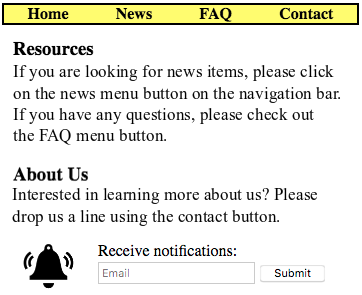
\includegraphics[scale=0.5]{accessibility_testing/figures/motivating-example/rendered-3.png}}
        \\ (c) Rendered page
    \end{minipage}
  
%    \begin{minipage}[c]{.6\columnwidth}\centering
%        (a) HTML code
%    \end{minipage}
%    \hfill
%    \begin{minipage}[c]{.5\columnwidth}\centering
%        (b) CSS declaration
%    \end{minipage}
%    \hfill    
%    \begin{minipage}[c]{.85\columnwidth}\centering
%        (c) Rendered page
%    \end{minipage}    
    \ \\ \caption{An example of an inaccessible web page.}
    \label{fig:acc-testing-motivating-example}
  \end{figure*}